\section{Mining for Cyberbullying Text}
\label{section:3.2}

The application of text mining tools, techniques and processes to the automatic detection of cyberbullying text is still a relatively new research area \cite{xu_fast_2012} \cite{xu_learning_2012}. There appears to be a clear trend where text mining approaches are supplemented with other techniques such as the analysis of the social graph of the bully and the victim or by determining the role played by each party in a cyberbullying incident. When training a classifier to identify documents of different types a ``bag of words'' approach is a commonly used method that uses the frequency of the occurrence of each word in a document as a feature used to help determine a documents class. One of the first mentions of a bag of words in this linguistic context was in the 1953 ``Distributional Structure'' paper by \citet{harris54}. The bag of words approach is at the heart of many attempts to automatically detect cyberbullying.

\citet{yin_detection_2009}, in ``Detection of Harassment on Web 2.0'' presents an approach to the detection of harassment that utilises content, sentiment and contextual features of documents. Using the Kongregate, Slashdot and MySpace datasets presented by Fundación Barcelona Media (FBM) for analysis at the CAW 2.0 workshop \cite{fundacion_barcelona_media_fbm_caw_2009}, the goal of this research was the identification of deprecating remarks. Three local features N-Grams, Foul words and Term Frequency - Inverse Document Frequency (TF-IDF) are used and local features are described as features that can be extracted directly from the text of the message. 

N-Grams are a contiguous sequence of n items from an extract of text or speech and in this occurrence the n-grams are words. For example, given a sequence of words ``The quick brown fox'' the following tri-grams, or sequences of three words, can be formed ``The quick brown'' and ``quick brown fox''. TF-IDF is a statistical measure of how important a given word is in a collection of documents. Each document is represented as a vector of words and each word is represented in the vector by a value that is indicative of its importance in predicting the class of the document. The TD-IDF weight for a word \textit{i} in document \textit{j} is given as: 

\begin{align}
	TFID{F}_{{ij}}=T{F}_{{ij}}\cdot ID{F}_{{i}}
\end{align}

Where \textit{TF} is a measure of a words importance in a document and is calculated as:

\begin{align}
	T{F}_{{{\dot{i}}j}}=\frac {{n}_{{ij}}}{{\Sigma }_{{k}}{n}_{{kj}}}
\end{align}

The number of times a word \textit{i} appears in a document \textit{j} is represented by ${{n}_{{ij}}}$ and ${{\Sigma }_{{k}}{n}_{{kj}}}$ is a count of all words in document \textit{j}. This means that the more times a word appears in a document the larger its value for \textit{TF} will get. The \textit{TF} weighting of a word in a document shows its importance within that single document. \textit{IDF} then shows the importance of a word within the entire collection of documents or corpus and is calculated as:

\begin{align}
	ID{F}_{{i}}={log{\frac {\mid{P}\mid}{\mid{\{{{p}_{{j}} \:: \: {t}_{{i}} \: \epsilon \: {p}_{{j}}}\}}\mid}}}
\end{align}

Where $\mid{P}\mid$ is the total number of documents in the corpus or collection and $\mid{\{{{p}_{{j}} \:: \: {t}_{{i}} \: \epsilon \: {p}_{{j}}}\}}\mid$ represents the number of documents in which the word, or term, ${t}_{{i}}$ appears. The nature of the \textit{IDF} value is such that terms which appear in a lot of documents will have a lower score or weight. This means terms that only appear in a single document, or in a small percentage of the documents, will receive a higher score. This higher score makes that word a good discriminator between posts \cite{yin_detection_2009}. 

In their research \citet{yin_detection_2009} used the libSVM \cite{CC01a} learner with a linear kernel as their classification tool with ten-fold cross validation. They found a combination of 1, 2 and 3 n-grams, foul or profane language and TF-IDF on their own did not perform very well. When applied separately to the three datasets F-Measure scores of less then 0.2 for n-grams and foul words and between 0.25 and 0.40 for TF-IDF were returned. When combined with sentiment features and contextual features a small improvement in F-Measure values was seen. When reviewing the dataset it was noticed that a lot of the posts classified as harassment contained foul language used in conjunction with pronouns, particularly second person personal pronouns such as ``you'', ``your'' and ``yourself''. To boost the effectiveness of these pronouns the sentiment features were captured together into three groups. The first group treated all second person pronouns together as a single term. The second group took all other pronouns together as a single term, for example, ``he'', ``she'', ``her'' etc. and the final group treated all foul words as a single term. The TF-IDF weighting of the combined terms was calculated for each group. It was identified, for contextual features, that the posts classified as harassment were ``different'' to their neighbouring posts so a cosine similarity between posts was calculated to assist in the identification of the bullying posts. The authors concluded that combining these sentiment and context feature to the earlier content features lead to an increase in F-Measure values to between approximately 0.3 and 0.44.

In ``Modelling the Detection of Textual Cyberbullying'', \citet{dinakar_modeling_2011}, a set of binary and multi-class classifiers, developed using a bag of words approach, are proposed for the detection of textual cyberbullying in a corpus of 50,000 YouTube comments. Unlike \citet{yin_detection_2009} a set of preprocessing steps were used on the comments including stemming, stop word removal and the removal of repeated characters for example ``lollllll''. Stemming is a process by which  derived or inflected  words are reduced to their stem, sometimes also called the base or root. Using the words stemming and stemmed as examples, these are both based on the word stem. The first algorithm proposed for a stemmer was by \citet{lovins_development_1968} in 1968. When processing natural language, or text, stop words are words which are filtered out of the corpus typically early on in the process \cite{rajaraman_mining_2011}. Stop word are usually what are called short function words or words with little or ambiguous meaning. Example of English stop words include ``the'', ``and'', ``at'', ``which'' etc.  After preprocessing, the YouTube comments were divided into several clusters representing different types of harassment, for example, physical appearance, sexuality, race and cultural and intelligence. From each cluster 1,500 comments were hand-annotated to verify that labels were correctly applied to each cluster. Comments that did not fit in any of the clusters were given a neutral label. Like \citet{yin_detection_2009} some general features of the text were used. Both TF-IDF weighted uni-grams and a list of profane words were used. In addition, the Ortony lexicon \cite{ortony_referential_1987} of words donating negative connotation, the positive words were stripped beforehand, and frequently occurring part of speech (POS) bi-grams were utilised. 

In their experiment set-up \citet{dinakar_modeling_2011} divided their datasets 50\% for training, 30\% for testing and 20\% for validation. A Naive Bayes classifier, as well as three supervised learning methods, were used to train a model. The supervised learner were Support Vector Machines (SVM), J48 which is a C4.5 based decision tree classifier and JRip a propositional rule learner. In the first experiment the models were trained on each dataset separately i.e. a binary classification task. In the second experiment the datasets were combined into a single dataset and the models were trained as a multi-class classifier. Rather than using accuracy alone in the assessment of the performance of the models developed Cohen's kappa statistic was also used. It was found that the binary classifiers developed performed much better than the multi-class classifier. It was also observed that whilst the JRip rule-based model gave the best accuracy with values as high as 80\% the SVM gave the best kappa statistic values ranging from 0.72 to 0.79 for the binary classifiers. \citet{kontostathis_chatcoder:_2009} also utilises the J48 classifier from Weka \cite{hall_weka_2009} when attempting to categorise predators and victims in grooming chat transcripts from Perverted Justice \cite{_perverted-justice.com_????} and ChatTrack \cite{bengel_chattrack:_2004}.

\citet{reynolds_using_2011} explicitly state that they wanted to avoid a bag of words approach. This was because the feature space of the bag of words approach can become very large, they wished to be able to produce the model in code and they wanted to be able to fully understand the reason a post was considered as cyberbullying. Having reached the conclusion that ``bad'' words, for example, swear words, profanities and offensive words, were a good indicator of cyberbullying a weighted dictionary of terms, built from the terms on www.noswearing.com, was generated. The weighting ranged from 100 to 500 depending on the deemed severity of the word. The dataset used was scrapped from the www.formspring.me website, a questions and answers style website, and labelled using Amazon Mechanical Turks. Using the bad word dictionary the contents of each message was then scored in several ways. Two datasets were created and in the first the count of bad words contained in each post, \textit{NUM}, was calculated and in the second a normalised count of the words, \textit{NORM}, was calculated to reflect the density of the bad words in each post. When calculating the normalised value the severity weight of each bad word was also considered. In additional \textit{SUM} and \textit{TOTAL} values were also calculated were SUM is the overall weighted average badness of a post taking into account the severity weighting of each word and TOTAL is the total number of words. In additional to the J48, JRip and SVM learners, which were also used in \cite{dinakar_modeling_2011}, IBK an instance based algorithm was also used. Using ten-fold cross validation the authors report that the NORM dataset outperformed the NUM dataset suggesting that the percentage of bad words in a post is more indicative of cyberbullying than a simple count of bad words. Overall the learners used, with the exception of SVM, were able to correctly identify 78.5\% of cyberbullying posts.

\citet{chen_detecting_2012} presents a two phase Lexical Syntactic Feature (LSF) based framework for the detection of offensive content and users. Their proposed system presents a new method of sentence offensiveness prediction based on the overall offensiveness of the words in the sentence. The offensive is measured using a lexicon constructed using \citet{xu_filtering_2010}, the Urban Dictionary, and a syntactic intensifier that adjusts a words offensiveness based on the context in the sentence. Words defined as being either strongly offensive and given a larger weighting, for example, profanities such as ``fuck''. Weakly offensive words, such as ``stupid'' or ``liar'', were given a smaller weighting. Words that were not offensive were given a neutral weighting. When a pejorative or obscenity is directed at a user, or semantically associated with another pejorative or obscenity, it is suggested that they become more offensive. For example, the word stupid would be considered more offensive when directed at a person, ``are you stupid'', opposed to referring to the latest console game ``it's a stupid game'' giving the word a larger intensifier value. Using this intensifier value the offensive value of a word is adjusted accordingly giving an overall sentence offensive value ${O}_{{s}}$ of:

\begin{align}
	{O}_{{s}}={\sum {{o}_{{w}}{I}_{{w}}}}
\end{align}

The offensiveness of a user is a combination of the aggregate of the sentence's offensiveness and the extraction of some of the users language styles. The dataset used was a corpus of over two million YouTube comments with minimal preprocessing. Six approaches were used to determine each sentence's offensive values including bag of words, 2-gram, 3-gram, 5-gram, an appraisal approach \cite{whitelaw_using_2005} and the newly proposed LSF approach. Recall, precision and F-Score, F-Measure, were used to evaluate each of the approaches. Also of interest to the authors was a measure of false positives, sentences erroneously scored as offensive, and false negatives, sentences that should have been scored as offensive but were not. A summary of how each approach performed is shown in Figure \ref{fig:chen_detecting_2012_01} where the Proposed LSF approach performed the best.

\begin{figure}[htbp]
	\centering
	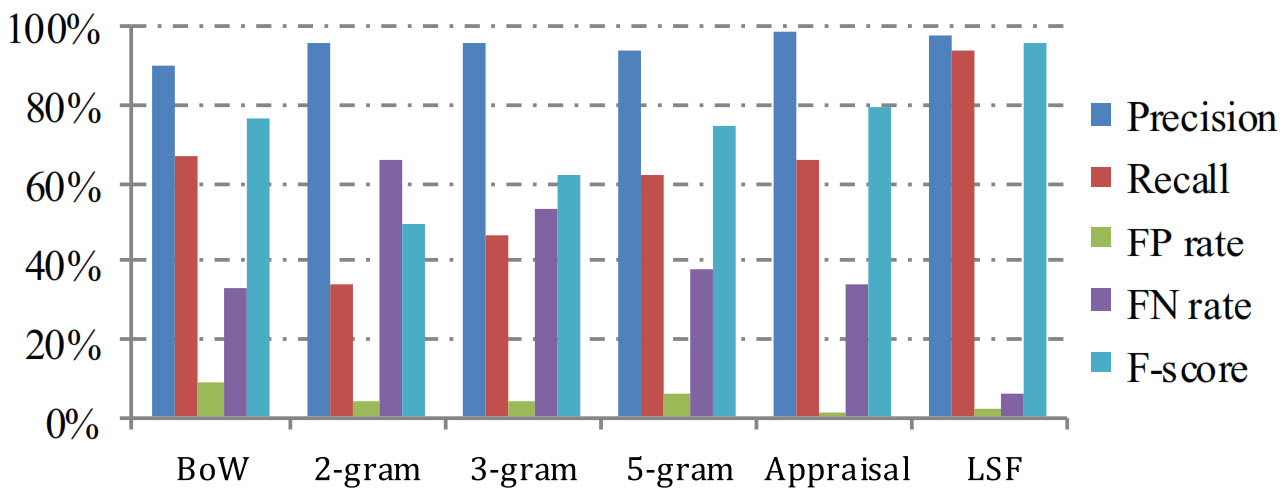
\includegraphics[width=0.75\textwidth]{Figures/Chapter3/chen_detecting_2012_01.jpg}
	\caption[Accuracies of sentence level offensiveness detection]{Accuracies of sentence level offensiveness detection \citet{chen_detecting_2012}}
	\label{fig:chen_detecting_2012_01}
\end{figure}

The calculation of an individual users offensiveness was a more complicated matter. A number of users, whose sentence offensiveness levels as calculated in phase one was uniformly distributed, next had their comments manually annotated as either offensive or not. Using Naive Bayes and SVM classifiers and ten-fold cross validation a number of experiments were then run to determine a user offensiveness estimation. The authors found that using both strongly offensive and weakly offensive words in the calculation achieved better results than the proposed LSH. However, on removing the strongly offensive words LSF proved a better predictor. In both cases, the learner that performed the best was SVM.

Like some of the previous papers reviewed \citet{dadvar_improving_2013} also used the content features of manually annotated comments collected from YouTube as well as cyberbullying features and user based features of the text. However, rather than use a bag of words and a TDIDF approach the numerical values for each feature was calculated. The first two content features used we have seen before. These are the number of profane words, taken from a dictionary of 414 words and the number of first and second person pronouns. Both of these features were normalised on the overall length of the comment. The third feature was a boolean feature called the profanity window which identified where a profanity was within a given window size, for example, two to five words, of a second person pronoun. The fourth feature was a normalised count of the number of emoticons. The final feature was the ratio of capital letters in the comment, to capture perceived shouting.  The cyberbullying features were the normalised number of bullying words based on a manually compiled dictionary of bullying words and also the length of the comment. It was proposed that bullying comments are typically shorter in length than not bullying comments. The final group of features used are user features. To exploit the knowledge already known about each user their historical content features were averaged to determine if there was a history of offensive language use. All the content features listed were considered in this calculation as well as the users age. Before processing stop word removal and stemming was applied. A SVM was used to classify the comments and precision, recall and F-Measure values were used to rate the performance of the model. The content based features were first used on their own to obtain a baseline. The content based features get an F-Measure value of 0.55. Next the cyberbullying features were also included and their inclusion saw an increase in the F-Measure value to 0.60. The user features were then added and this resulted in an F-Measure value of 0.64 which led the authors to conclude that the inclusion of user features lead to an increase in the detection of cyberbullying accuracy.

\citet{xu_learning_2012} say that the computational study of cyberbullying is, except for a few exceptions, largely unexplored. Using simple logic based on manual inspection of a Twitter dataset they calculate that there are probably upwards of 50,000 English bullying tweets a day. They outline three approaches that could be used in the detection of cyberbullying. The first is a Natural Language Processing (NLP) task which uses a sample dataset of tweets that has been keyword filtered to contain the terms ``bully'', ``bullied'' and ``bullying''. 1,762 sample tweets were hand annotated and no pre-processing, such as stop word removal or stemming, was performed but the data was case folded \cite{settles_closing_2011}, user names were anonymised, and URLs were replaced with the ``HYPERLINK'' token. Emoticons and Hashtags were also treated as tokens. Following this processing three feature representations, uni-grams (1g), uni-grams and bi-grams(1g2g) and part of speech (POS) coloured uni-grams and bi-grams (1g2gPOS) were created. Four common text classifiers, Näive Bayes, SVM with linear kernel, SVM with RBF kernel and Logistic Regression, were trained on dataset sizes ranging from 100 to 1,500 tweet and then tested using tweets that were held back. Although SVM(linear) + 1g2gPOS achieved an accuracy of 81.6\%  it was decided that SVM(linear) + 1g2g, 81.3\% accuracy on the training data and F-measure 0.77 on the test data, was preferred due to its simplicity. Of all the classifiers used, Naive Bayes performed the worst.

The second approach suggested by \citet{xu_learning_2012} is based around the role a user takes in a cyberbullying incident. These roles, and their relationship, is shown in Figure \ref{fig:xu_learning_2012_01}:

\begin{figure}[htbp]
	\centering
	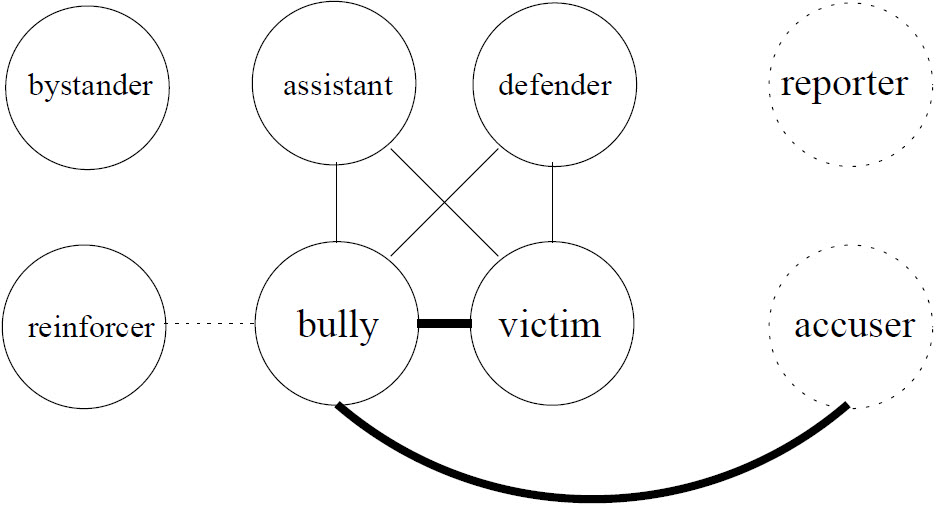
\includegraphics[width=0.75\textwidth]{Figures/Chapter3/xu_learning_2012_01.jpg}
	\caption[Roles taken in a cyberbullying incident]{Roles taken in a cyberbullying incident \citet{xu_learning_2012}}
	\label{fig:xu_learning_2012_01}
\end{figure}

The role taken by the bully and the victim are apparent and need not be examined further. The bullying role is supported by the assistant role and reinforcer role. Though they did not start the bullying the assistant joins in and adds further bullying comments The reinforcer is seen to approve, maybe by liking the bully's post, but does not directly join in. The defender, reporter and accuser roles support the victim. The defender will stand up for the victim, maybe by adding positive comments and also by standing up for the victim. The accuser, however, will go a step further and might confront the bully about the offending comment and point out that they are bullying the victim. The reporter brings the bullying content to the attention of a parent or other authoritative figure. The bystander sees the post and does nothing. The primary interaction is between the bully and the victim but the strength of the line from the accuser to bully is indicative that the confrontation of the bully by the accuser is equally important. 

Four of the most frequently observed roles are targeted Accuser (A), Bully (B), Reporter (R) and Victim (V). The other roles were merged into a single generic role of Other (O). Two tasks were then defined. The first is to identify the author of the tweet which is held in an AUTHOR token. The second is to label each person mentioned in the tweet with one of the bullying roles. Following a manual annotation exercise and using the same classifiers and training techniques as before SVM(linear) + 1g2g gave the best results in the first task. The second task compared the performance of a Conditional Random Field (CRF) classifier against the SVM(linear) to correctly identify the various roles. Once again the data was manually annotated and it was found that for this task the CRF outperformed SVM with an accuracy of 87\% and an overall F-Measure of 47\%. It was discussed that the performance values for precision and recall were low because the tweets were short in length and considered noisy.

Sentiment analysis was the next task undertaken. It was decided to focus on whether a tweet, previously identified as bullying, could be considered as teasing. Hand annotating the tweets from the initial text categorisation task and using the same feature representations and classifiers SVM(linear) + 1g2g again gave the best accuracy performance of 89\%. However, overall, nearly half of the teasing example were misclassified. The lack of emoticons or tokens, and the inconsistency of their use, where they are used indiscriminately in both bullying and not bullying tweets was suggested as a possible reason why the overall performance was poor. Another reason suggested was the lack of standardisation in the spelling of the token or the representation of the emoticon.  

Finally in an effort to understand the main topics from the cyberbullying tweets a collapsed Gibbs sampling implementation of Latent Dirichlet Allocation (LDA) \cite{griffiths_finding_2004} was run. Six topics of interest highlighted by the authors are feelings, suicide, family, school, verbal bullying and physical bullying.


A novel approach to the detection of cyberbullying by using gender information is suggested by \citet{dadvar_improved_2012} . Referring to work by \citet{argamon_gender_2003} and \citet{chisholm_cyberspace_2006} the authors investigated the differing bullying vocabularies of males, who tend to use profanities and threatening behaviour, and females, who use a more relational aggression such as social exclusion or by ganging up on an individual. This was shown to be true as seen in Figure \ref{fig:dadvar_improved_2012_01}. Using supervised learning on a corpus where the gender of the author was known, the dataset was separated into male and female subsets and the features of each set of posts are extracted. Profane words are treated by calculating their ratio in each post and then normalising. Second person pronouns are again considered important and treated separately to all other pronouns. A TF-IDF of all the words in the post was also calculated. The authors of the paper found that incorporating gender specific features achieved better overall detection accuracy with a 39\% increase in precision, 6\% increase in recall and 15\% improvement in the F-Measure.


\begin{figure}[htbp]
	\centering
	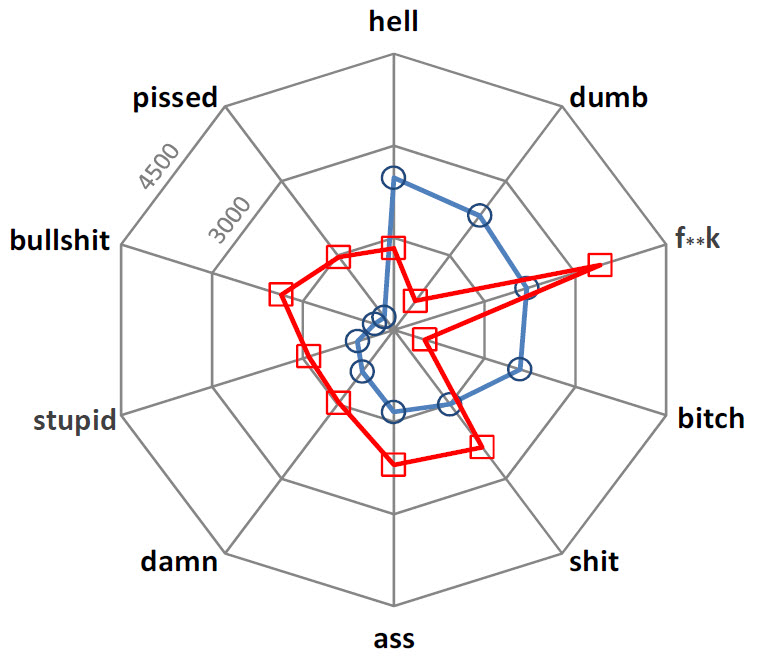
\includegraphics[width=0.75\textwidth]{Figures/Chapter3/dadvar_improved_2012_01.jpg}
	\caption[Top ten profane words for male and female authors]{Top ten profane words for male (square) and female (circle) authors \citet{dadvar_improved_2012}}
	\label{fig:dadvar_improved_2012_01}
\end{figure}
 

\citet{nahar_effective_2013} suggests a two phase approach  to identify cyberbullying instigators and victims by graphing the cyberbullying network and by using a ranking algorithm. In phase one harmful messages are detected using a weighted TF-IDF scheme on bullying features, like a bad word dictionary, and an LDA topic modelling approach which, as previously seen, can be used to understand the underlying semantic topics (for example bullying). The second phase involves building a weight directed graph model of the users social networks to determine who the victims are and who the predators are. Each user is given a predator and victim rank based on the number of harmful messages sent or received. A predator is a user that sends messages with harmful words to users with a higher victim score, a victim is a user that receives messages from users with higher predator scores. Using the users predator and victim ranking in conjunction with the message analysis results from the first phase it was possible to more accurately predict real instances of cyberbullying. Figure \ref{fig:nahar_effective_2013_01} shows an example weighted graph where \textit{u1} has been identified as a predator and \textit{u2} a victim based on the number of harmful messages sent or received.

\begin{figure}[htbp]
	\centering
	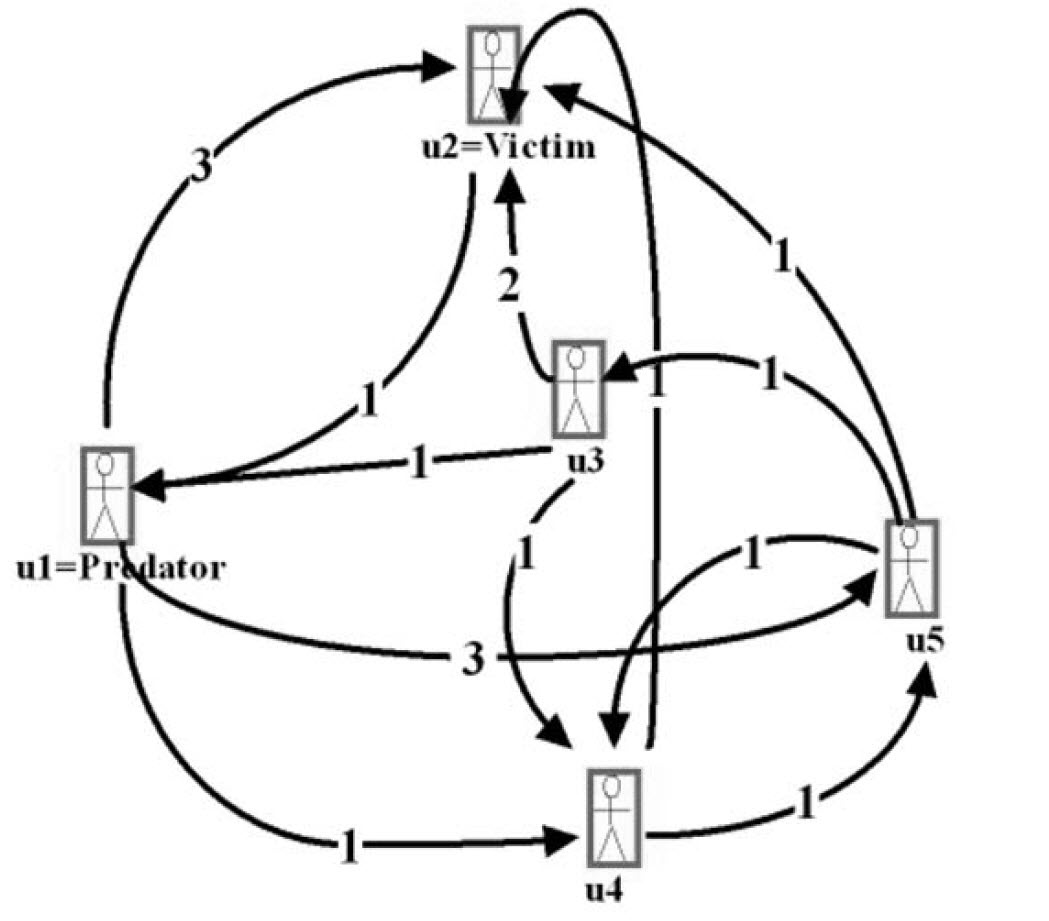
\includegraphics[width=0.75\textwidth]{Figures/Chapter3/nahar_effective_2013_01.jpg}
	\caption[Weighted graph model identifying predators and victims]{Weighted graph model identifying predators and victims \citet{nahar_effective_2013}}
	\label{fig:nahar_effective_2013_01}
\end{figure}

The corpora used were the FBM MySpace, Kongregate and Slashdot datasets from CAW 2009 \cite{fundacion_barcelona_media_fbm_caw_2009}. The data was deemed to be noisy and was preprocessed to increase the quality and the effectiveness of the analytical steps. The text was converted to lower case then stemming and stop words removal was applied before hyperlinks and extra characters were removed. As seen in other works, three types of semantic features, all second person pronouns, all other pronouns and foul words were defined. A weighted TF-IDF scheme was used with the foul words weighted by a factor by two. Finally, an LDA model was used, and the top features generated were selected. The words generated under the bullying, and not bullying topics were extracted and ranked. A linear kernel SVM classifier was used to generate the model. The weighted TF-IDF results were compared against the previous research baseline values, by the same authors \cite{nahar_sentiment_2012}, and also against the LDA features. The weighted TF-IDF outperformed the baseline significantly. On the Slashdot an MySpace datasets it was nearly by a factor of three with an F-Measures of 0.30 and 0.31 for the former and 0.87 and 0.92 for the latter.  Overall it was considered that weighted TF-IDF outperformed all other methods.

The final paper to be reviewed in this section was \citet{kontostathis_detecting_2013} where a number of experiments are performed to identify terms that are indicative of cyberbullying. The dataset used was one that was manually scrapped from the www.formspring.me social media site where users interact using a question and answer model. The dataset was labelled using the Amazon Mechanical Turk service with posts identified as cyberbullying labelled as yes and not bullying posts labelled as no. Approximately 11\% of posts, or 1,185 out of 10,685, were identified as containing content that could be considered cyberbullying. The first experiments utilised a bag of words approach that the authors consider as simple and transparent. The only pre-processing performed was the conversion of all letters to lower case and the removal of all numeric characters and special characters. It was identified that this could lead to the loss of the emphasis as capital letters can be used to show displeasure. The removal of the special characters would also lead to emoticons being removed which are used to show emotions. No other pre-processing was performed giving 15,713 unique terms which gave a term by document matrix of 10,685 x 15,713 where the intersection of rows and columns represented the number of times a term appeared in a particular post. As discussed previously it was determined that ``bad'' words are a likely predictor of cyberbullying. A dictionary of bad words was constructed using the terms on the www.noswearing.com website. Each term in the bad word dictionary was then used to query the 10,685 posts returning the number of times each word appears in each post. After all the words in the dictionary had been queried any posts that returned zero bad words were discarded. The remaining posts were sorted by their overall bad word occurrence count. The number of true positive posts in the top 10, 20, 30, 100 and 500 sorted posts was also noted to identify the terms that yielded the highest top  scores. Another similar round of context based experiments was also run using the 1,185 identified bullying posts. 

The outcome from the first set of queries was to assist in developing another set of query terms that could be used to predict cyberbullying. Precision, recall and f-measure were used to determine the performance of this first set of queries. The result of this analysis was four groups of terms from the bad word dictionary. The first set of words were representative of the terms that results in a precision value of greater than 0.75 and it was found that twenty five terms met this criteria. The next group was made up of 39 terms that achieved a true positive rate for recall of greater than 0.50. The third group of term were representative of words that had at least five posts in the top ten list of posts when sorted by bad word rating of which there were 48 terms. The final content based group consisted of all the terms in the bad word dictionary. A similar analysis was performed on the results of the context queries. There were seven posts with a precision of greater than 0.75 and the words from these posts were used to form the first context based group of words. The second group of context based words was made up of the terms in the top ten queries that had the highest number of true positives. the final context group contained the words of posts that had at least nine true positives in the top ten ranked documents. These four content based and three context based queries were then run against the data and their results were analysed. The authors found that the bad words content queries, F-Measure 0.49 to 0.57, outperformed the context queries, F-Measure 0.28 - 0.45, even though the context queries contained helper and filler words which it was assumed would help. Whilst it was found that precision values were high, recall values did suffer and while the longer content based queries were effective this was at the cost of performance.

This completes the review of approaches that can be used to mine text posted on social network sites for cyberbullying content. During the course of this review it was clear that a number of issues or obstacles reappeared again and again throughout all the papers reviewed. The next section will give a brief overview of these issues and some of the suggested solutions. The topics covered include anonymity, the availability of suitable datasets, classification or labelling and handling class imbalance.
